
% per ottenere biliardo.svg:
% $ pdflatex biliardo.tex && pdf2svg biliardo.pdf biliardo.svg
\documentclass[tikz]{standalone}

\begin{document}

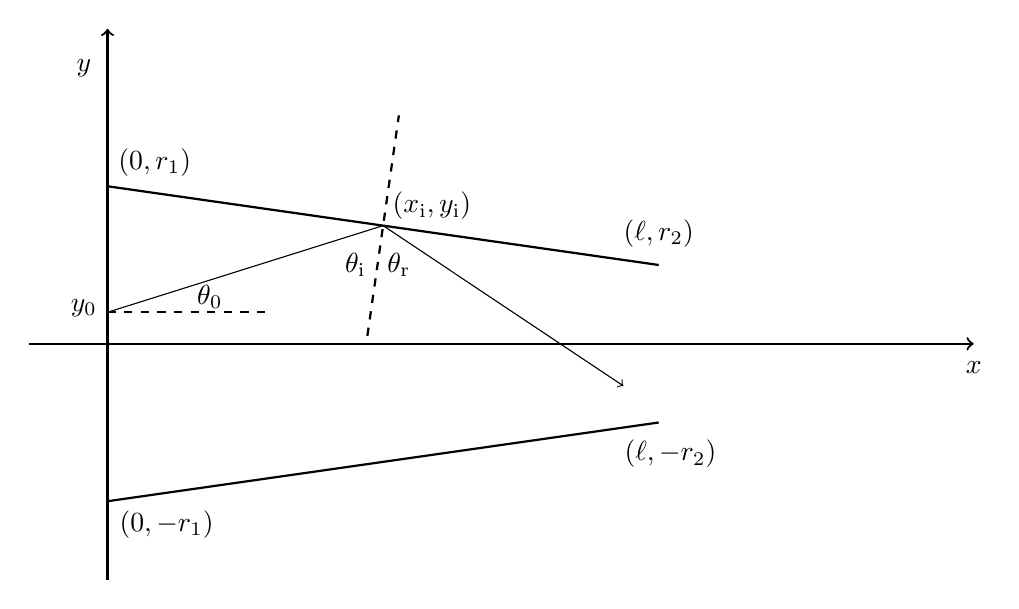
\begin{tikzpicture}

  \draw[thick, <->] (11,0) -- (0,0) -- (0, 4);
  \draw[thick] (0,0) -- (0, -3);
  \draw[thick] (0,0) -- (-1, 0);
  \node at (11,-0.3) {$x$};
  \node at (-0.3, 3.5) {$y$};
  \draw[thick] (0,2) -- (7,1);
  \node at (0.6,2.3) {$(0,r_1)$};
  \node at (7,1.4) {$(\ell,r_2)$};
  \draw[thick] (0,-2) -- (7,-1);
  \node at (0.75,-2.3) {$(0,-r_1)$};
  \node at (7.15,-1.4) {$(\ell,-r_2)$};
  \draw[thick,dashed] (3.3,0.1) -- (3.7,2.9);
  \draw (0,0.4) -- (3.5,1.5);
  \draw[thick,dashed] (0,0.4) -- (2,0.4);
  \node at (-0.3,0.45) {$y_0$};
  \node at (1.3,0.6) {$\theta_0$};
  \node at (3.15,1) {$\theta_\mathrm{i}$};
  \node at (3.7,1) {$\theta_\mathrm{r}$};
  \draw [->] (3.5,1.5) -- (6.552, -0.536);
  \node at (4.12,1.75) {$(x_\mathrm{i},y_\mathrm{i})$};

\end{tikzpicture}

\end{document}

